%\documentclass[9pt]{beamer}
%\usefonttheme[onlylarge]{structurebold}

\documentclass[handout]{beamer}
\usefonttheme[onlylarge]{structurebold}
  \usepackage{pgfpages}
\mode<handout>
\pgfpagesuselayout{4 on 1}[letterpaper,border shrink=5mm]

\hypersetup{
  bookmarks = false,
  colorlinks,
  citecolor = red,
  linkcolor=blue,
  pdfpagemode=none,
  pdfstartview={Fit},
  pdftitle={},
  pdfauthor={Michael E. Waugh},
  pdfkeywords={} }
  \setbeamertemplate{navigation symbols}{}

\mode<presentation> {
  \usetheme{boxes}
  % or ...

  \setbeamercovered{transparent}
  % or whatever (possibly just delete it)
}

\setbeamertemplate{itemize subitem}[circle]
\setbeamerfont{frametitle}{size= \large}
\setbeamerfont{ framesubtitle }{size = \footnotesize}
\setbeamertemplate{frametitle}
{
\medskip
\smallskip
{\textsf{\underline{\insertframetitle\phantom{))))))))}}}}}


\usepackage[english]{babel}
\usepackage{wasysym}

\addfootbox{}{\hspace{6cm}\tiny {Trade Imbalances---Economics of Global Business, Revised: \today}}%

\title[NYU Stern] % (optional, use only with long paper titles)
{\Large \Large Trade Imbalances}

\author[Michael Waugh] % (optional, use only with lots of authors)
{\bf{\Large}}%

\date[] % (optional)

\subject{Talks}

\begin{document}


\begin{frame}
  \titlepage
\end{frame}

\begin{frame}[t]
\frametitle{Big Picture}
\bigskip
\begin{itemize}
\item In an open economy
\begin{itemize}
\medskip
\item spending need not equal output
\medskip
\item saving need not equal investment
\end{itemize}
\bigskip
\item Think about your economic life\ldots
\begin{itemize}
\medskip
\item Does your spending equal your income?
\medskip
\item What does it imply when it does not? Saver? Borrower?
\end{itemize}
\end{itemize}
\bigskip
\end{frame}

%%%%%%%%%%%%%%%%%%%%%%%%%%%%%%%%%%%%%%%%%%%%%%%%%%%%%%%%%%%%%%%%%%%%%%%%%%%%%%%%%%%%%%%%%%%%%%%%%%
%%%%%%%%%%%%%%%%%%%%%%%%%%%%%%%%%%%%%%%%%%%%%%%%%%%%%%%%%%%%%%%%%%%%%%%%%%%%%%%%%%%%%%%%%%%%%%%%%%

\begin{frame}[t]
\frametitle{Open economy demand for goods and services}
\begin{itemize}
\item Expenditure Components
\begin{itemize}
\medskip
\item C $=$ consumer demand for goods and services
\medskip
\item I $=$ demand for investment goods.
\medskip
\item G $=$ government demand for goods and services
\medskip
\item EX $=$ foreign demand for home goods and services
\medskip
\item IM $=$ domestic demand for foreign goods and services
\end{itemize}
\end{itemize}
\bigskip
\end{frame}

%%%%%%%%%%%%%%%%%%%%%%%%%%%%%%%%%%%%%%%%%%%%%%%%%%%%%%%%%%%%%%%%%%%%%%%%%%%%%%%%%%%%%%%%%%%%%%%%%%
%%%%%%%%%%%%%%%%%%%%%%%%%%%%%%%%%%%%%%%%%%%%%%%%%%%%%%%%%%%%%%%%%%%%%%%%%%%%%%%%%%%%%%%%%%%%%%%%%%

\begin{frame}[t]
\frametitle{Savings, Investment, Net Exports I}
Recall\ldots
\begin{eqnarray*}
Y = C + I +  G + NX.
\end{eqnarray*}
Then rearranging \ldots
\begin{eqnarray*}
\small S &= \underbrace{Y - C}_{\small \mbox{Private \ Savings}} \ \ \ \ - \underbrace{\bar G}_{\small \mbox{Public\ Savings}} \\
\\
\\
&= I + NX
\end{eqnarray*}
\end{frame}

%%%%%%%%%%%%%%%%%%%%%%%%%%%%%%%%%%%%%%%%%%%%%%%%%%%%%%%%%%%%%%%%%%%%%%%%%%%%%%%%%%%%%%%%%%%%%%%%%%
%%%%%%%%%%%%%%%%%%%%%%%%%%%%%%%%%%%%%%%%%%%%%%%%%%%%%%%%%%%%%%%%%%%%%%%%%%%%%%%%%%%%%%%%%%%%%%%%%%

\begin{frame}[t]
\frametitle{Savings, Investment, Net Exports II}
Then rearranging again\ldots
\begin{eqnarray*}
\small S - I = \underbrace{NX}_{\small \mbox{international borrowing/lending}}
\end{eqnarray*}\\
\bigskip
Think about if net exports are positve\ldots
\begin{itemize}
\smallskip
\item Selling more goods than buying\ldots how is this possible\ldots Then you must be a net \textbf{lender} to the rest of the world.
\end{itemize}
\bigskip
If net exports are negative\ldots
\begin{itemize}
\smallskip
\item Buying more goods than selling\ldots how is this possible\ldots Then you must be a net \textbf{borrowing} from the rest of the world.
\end{itemize}
\end{frame}

%%%%%%%%%%%%%%%%%%%%%%%%%%%%%%%%%%%%%%%%%%%%%%%%%%%%%%%%%%%%%%%%%%%%%%%%%%%%%%%%%%%%%%%%%%%%%%%%%%
%%%%%%%%%%%%%%%%%%%%%%%%%%%%%%%%%%%%%%%%%%%%%%%%%%%%%%%%%%%%%%%%%%%%%%%%%%%%%%%%%%%%%%%%%%%%%%%%%%

\begin{frame}[t]
\frametitle{Savings, Investment, Net Exports III}
Then rearranging again\ldots
\begin{eqnarray*}
\small S - I = \underbrace{NX}_{\small \mbox{Trade Balance}}
\end{eqnarray*}\\
\bigskip
Key point\ldots
\begin{itemize}
\smallskip
\item Trade balance tells us about net international capital flows.
\medskip
\item If running a trade deficit, then this implies a country is a net borrower!!!!
\end{itemize}
\end{frame}

%%%%%%%%%%%%%%%%%%%%%%%%%%%%%%%%%%%%%%%%%%%%%%%%%%%%%%%%%%%%%%%%%%%%%%%%%%%%%%%%%%%%%%%%%%%%%%%%%%
%%%%%%%%%%%%%%%%%%%%%%%%%%%%%%%%%%%%%%%%%%%%%%%%%%%%%%%%%%%%%%%%%%%%%%%%%%%%%%%%%%%%%%%%%%%%%%%%%%

\begin{frame}[t]
\frametitle{Savings and Investment in Small Open Economy}
\begin{itemize}
\item Production
\begin{eqnarray*}
\bar Y = \mbox{F}(\bar K, \bar L).
\end{eqnarray*}
\item Consumption
\begin{eqnarray*}
C = \beta \times (Y - T), \quad \mbox{where} \quad \beta \in (0,1).
\end{eqnarray*}
\item Investment function is:
\begin{eqnarray*}
I = I(r)
\end{eqnarray*}
\item Government policy
\begin{eqnarray*}
G = \bar G \ \ \ \ T = \bar T
\end{eqnarray*}
\end{itemize}
\end{frame}

%%%%%%%%%%%%%%%%%%%%%%%%%%%%%%%%%%%%%%%%%%%%%%%%%%%%%%%%%%%%%%%%%%%%%%%%%%%%%%%%%%%%%%%%%%%%%%%%%%
%%%%%%%%%%%%%%%%%%%%%%%%%%%%%%%%%%%%%%%%%%%%%%%%%%%%%%%%%%%%%%%%%%%%%%%%%%%%%%%%%%%%%%%%%%%%%%%%%%

\begin{frame}[t]
\frametitle{Supply of Savings}
\begin{center}
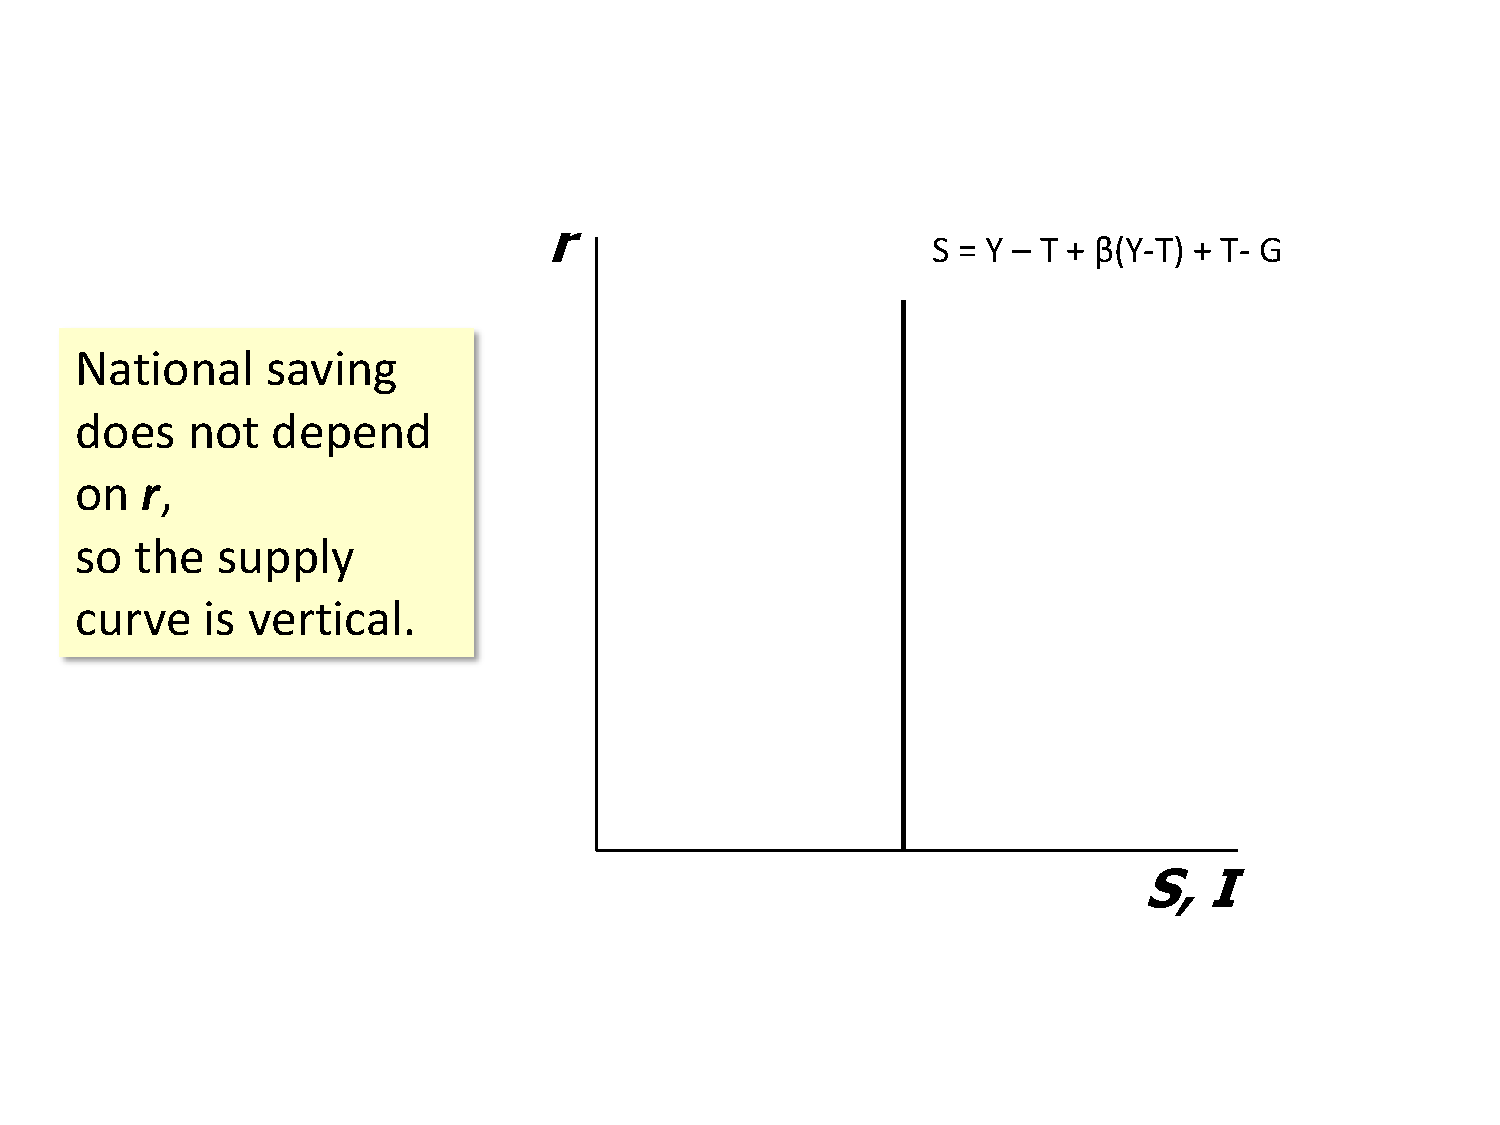
\includegraphics[height=3.1in,width=4.25in]{savins_funds.pdf}
\end{center}
\end{frame}

%%%%%%%%%%%%%%%%%%%%%%%%%%%%%%%%%%%%%%%%%%%%%%%%%%%%%%%%%%%%%%%%%%%%%%%%%%%%%%%%%%%%%%%%%%%%%%%%%%
%%%%%%%%%%%%%%%%%%%%%%%%%%%%%%%%%%%%%%%%%%%%%%%%%%%%%%%%%%%%%%%%%%%%%%%%%%%%%%%%%%%%%%%%%%%%%%%%%%

\begin{frame}[t]
\frametitle{Assumptions about capital flows}
\begin{itemize}
\item[1.] Domestic \& foreign assets are perfect substitutes (same risk, maturity, etc.)

\item[2.]  Perfect capital mobility: No restrictions on international trade in assets

\item[3.]  Economy is small: \\
Cannot affect the world interest rate, denoted $r^*$
\end{itemize}
\bigskip
$1.$ and $2.$ imply that domestic $r = r^*$ always.\\
\bigskip
$3.$ implies actions in home economy do not affect $r^*$.
\end{frame}

%%%%%%%%%%%%%%%%%%%%%%%%%%%%%%%%%%%%%%%%%%%%%%%%%%%%%%%%%%%%%%%%%%%%%%%%%%%%%%%%%%%%%%%%%%%%%%%%%%
%%%%%%%%%%%%%%%%%%%%%%%%%%%%%%%%%%%%%%%%%%%%%%%%%%%%%%%%%%%%%%%%%%%%%%%%%%%%%%%%%%%%%%%%%%%%%%%%%%

\begin{frame}[t]
\frametitle{Investment in Open Economy}
\begin{center}
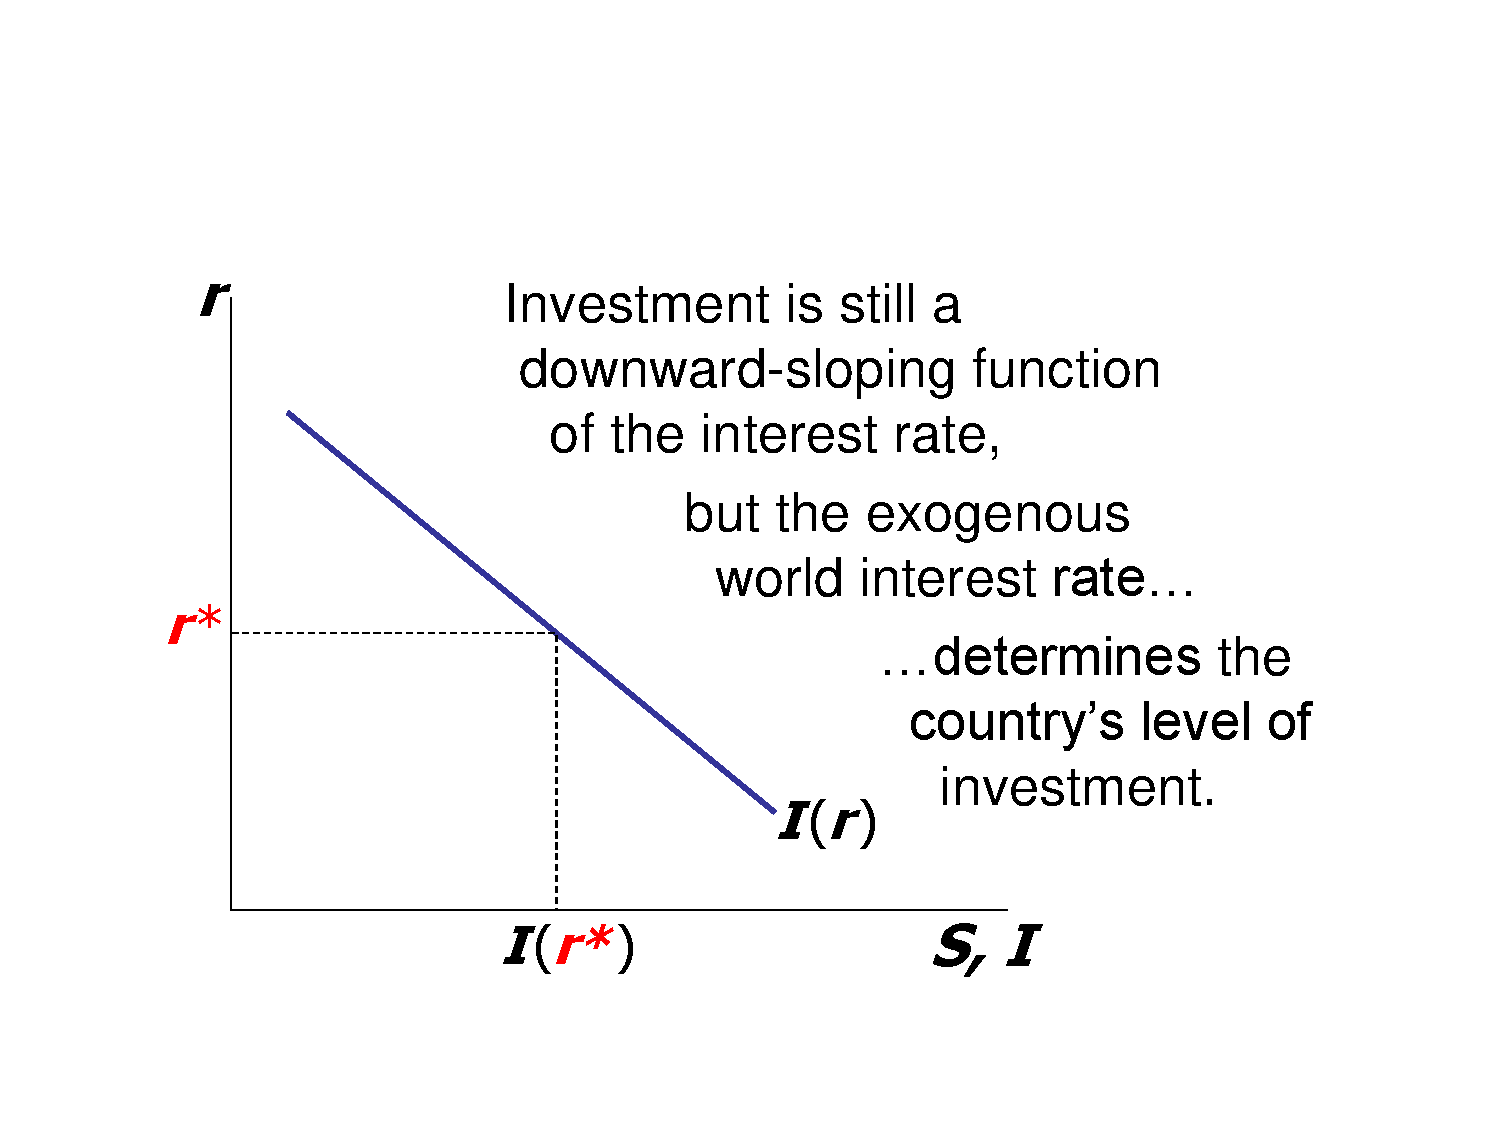
\includegraphics[height=3.1in,width=4.25in]{ch6_investment_curve.pdf}
\end{center}
\end{frame}

%%%%%%%%%%%%%%%%%%%%%%%%%%%%%%%%%%%%%%%%%%%%%%%%%%%%%%%%%%%%%%%%%%%%%%%%%%%%%%%%%%%%%%%%%%%%%%%%%%
%%%%%%%%%%%%%%%%%%%%%%%%%%%%%%%%%%%%%%%%%%%%%%%%%%%%%%%%%%%%%%%%%%%%%%%%%%%%%%%%%%%%%%%%%%%%%%%%%%

\begin{frame}[t]
\frametitle{Equilibrium in Closed Economy}
\begin{center}
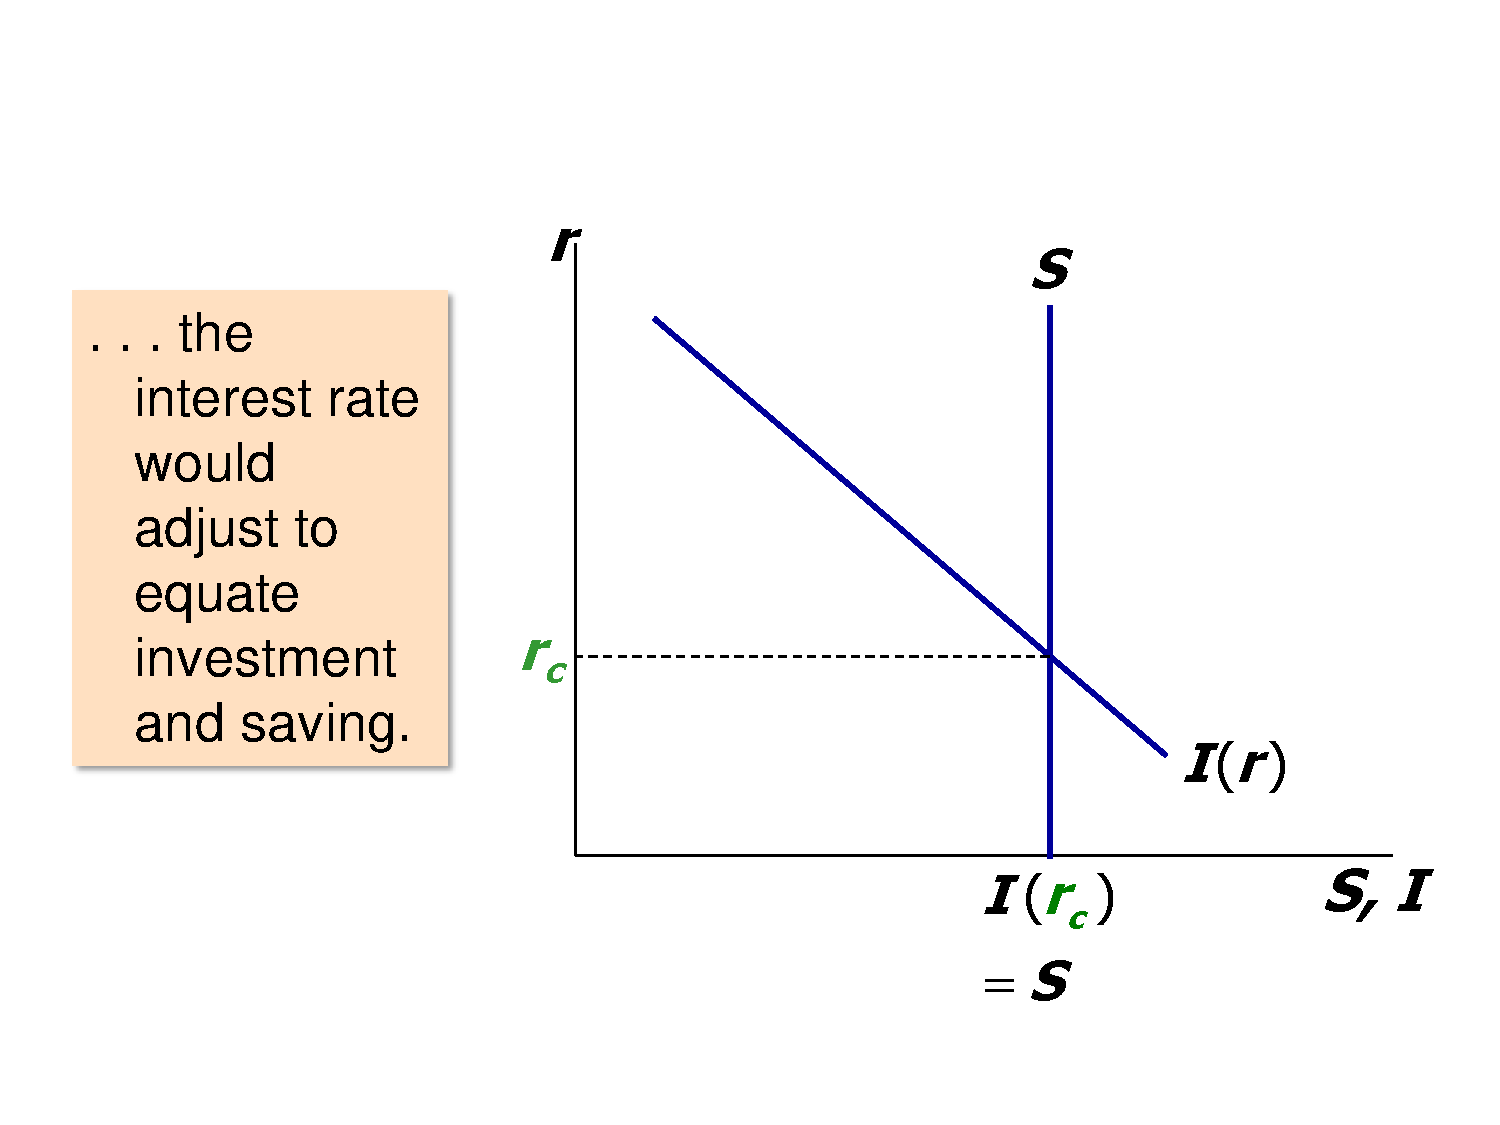
\includegraphics[height=3.1in,width=4.25in]{ch6_investment_curve_2.pdf}
\end{center}
\end{frame}

%%%%%%%%%%%%%%%%%%%%%%%%%%%%%%%%%%%%%%%%%%%%%%%%%%%%%%%%%%%%%%%%%%%%%%%%%%%%%%%%%%%%%%%%%%%%%%%%%%
%%%%%%%%%%%%%%%%%%%%%%%%%%%%%%%%%%%%%%%%%%%%%%%%%%%%%%%%%%%%%%%%%%%%%%%%%%%%%%%%%%%%%%%%%%%%%%%%%%

\begin{frame}[t]
\frametitle{Equilibrium in Open Economy}
\begin{center}
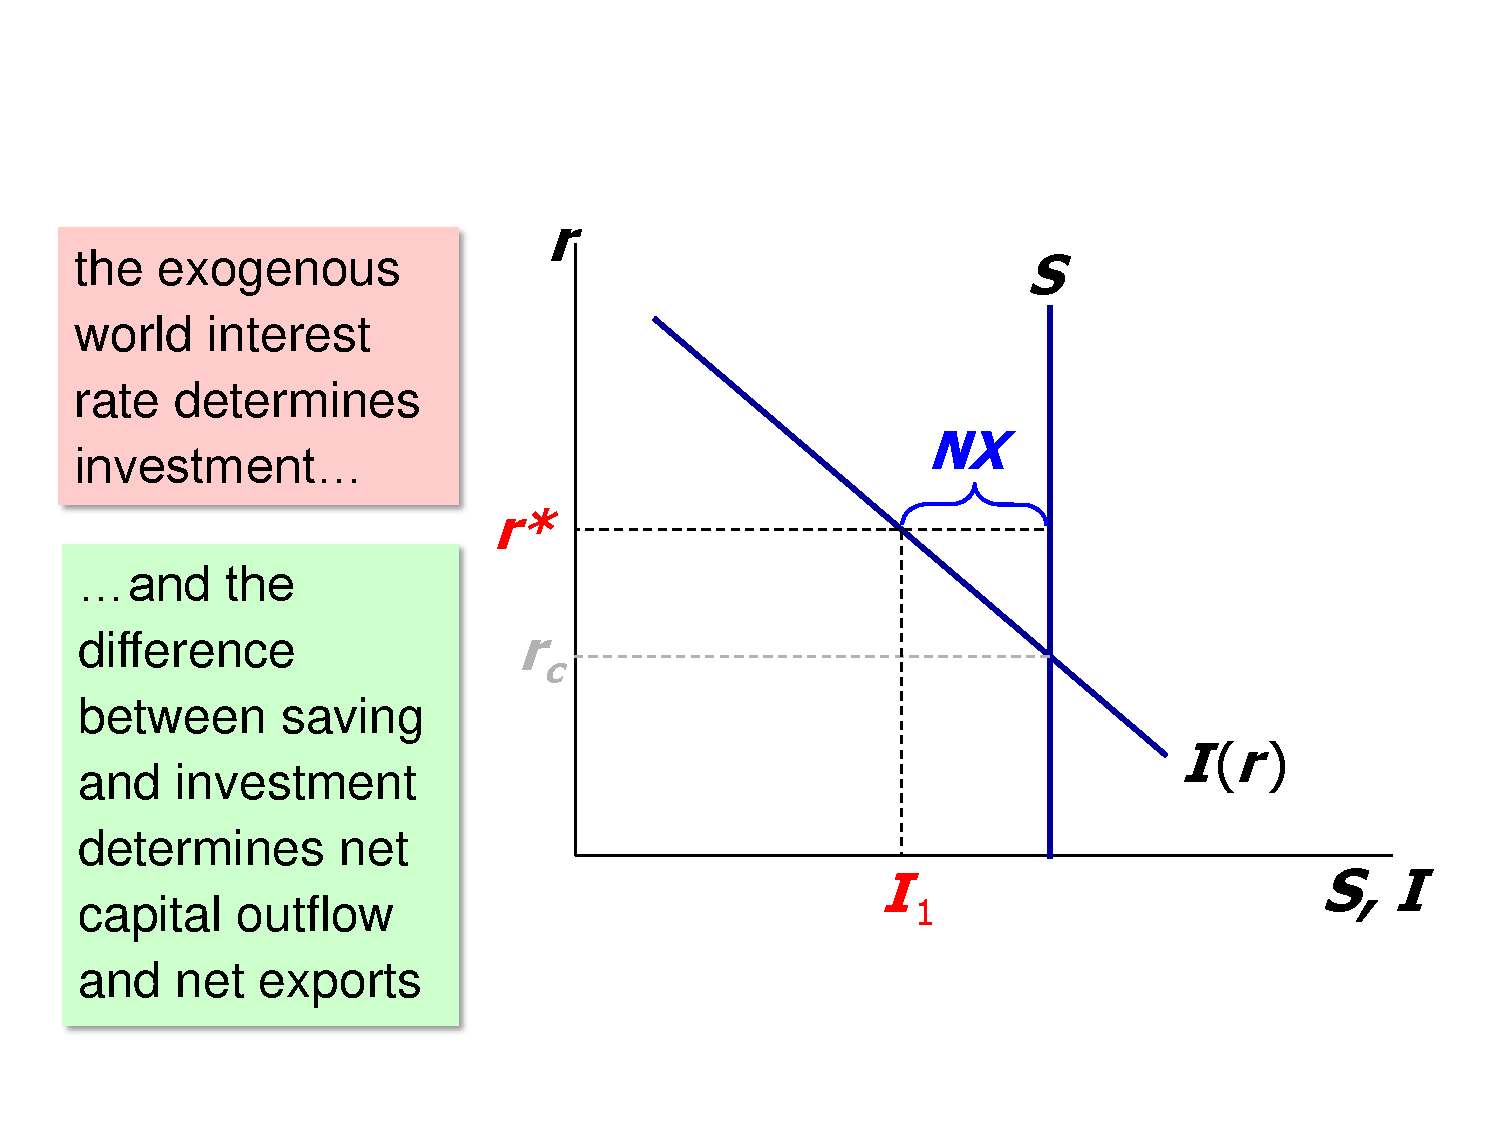
\includegraphics[height=3.1in,width=4.25in]{ch6_investment_curve_3.pdf}
\end{center}
\end{frame}

%%%%%%%%%%%%%%%%%%%%%%%%%%%%%%%%%%%%%%%%%%%%%%%%%%%%%%%%%%%%%%%%%%%%%%%%%%%%%%%%%%%%%%%%%%%%%%%%%%
%%%%%%%%%%%%%%%%%%%%%%%%%%%%%%%%%%%%%%%%%%%%%%%%%%%%%%%%%%%%%%%%%%%%%%%%%%%%%%%%%%%%%%%%%%%%%%%%%%

\begin{frame}[t]
\frametitle{Several things worth thinking about\ldots}
\begin{itemize}
\item[1.] How does fiscal policy at home affect the trade deficit?
\bigskip
\item[2.] How do changes in the world interest rate affect the trade deficit?
\bigskip
\item[3.] How do changes in investment demand affect the trade deficit?
\end{itemize}
\end{frame}

%%%%%%%%%%%%%%%%%%%%%%%%%%%%%%%%%%%%%%%%%%%%%%%%%%%%%%%%%%%%%%%%%%%%%%%%%%%%%%%%%%%%%%%%%%%%%%%%%%
%%%%%%%%%%%%%%%%%%%%%%%%%%%%%%%%%%%%%%%%%%%%%%%%%%%%%%%%%%%%%%%%%%%%%%%%%%%%%%%%%%%%%%%%%%%%%%%%%%

\begin{frame}[t]
\frametitle{The US Trade Deficit}
\begin{center}
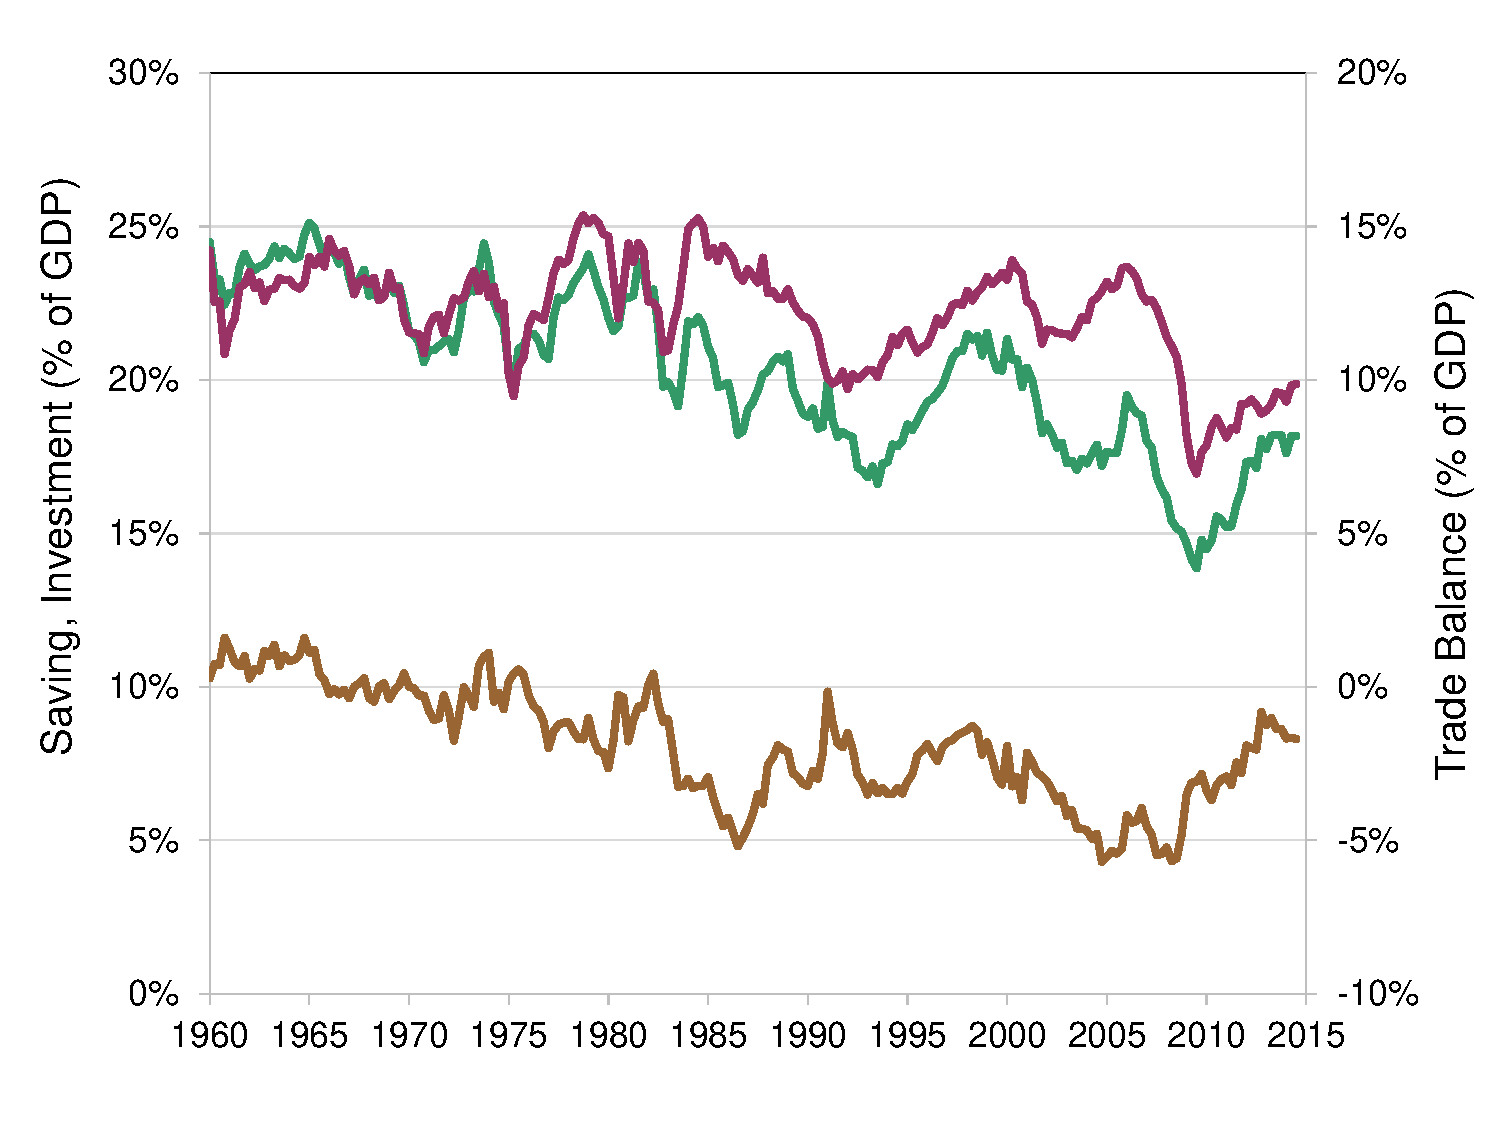
\includegraphics[height=3.1in,width=4.25in]{us_trade_deficit.pdf}
\end{center}
\end{frame}

%%%%%%%%%%%%%%%%%%%%%%%%%%%%%%%%%%%%%%%%%%%%%%%%%%%%%%%%%%%%%%%%%%%%%%%%%%%%%%%%%%%%%%%%%%%%%%%%%%
%%%%%%%%%%%%%%%%%%%%%%%%%%%%%%%%%%%%%%%%%%%%%%%%%%%%%%%%%%%%%%%%%%%%%%%%%%%%%%%%%%%%%%%%%%%%%%%%%%

\begin{frame}[t]
\frametitle{US NX and Government Budget Deficit (\% of GDP)}
\begin{center}
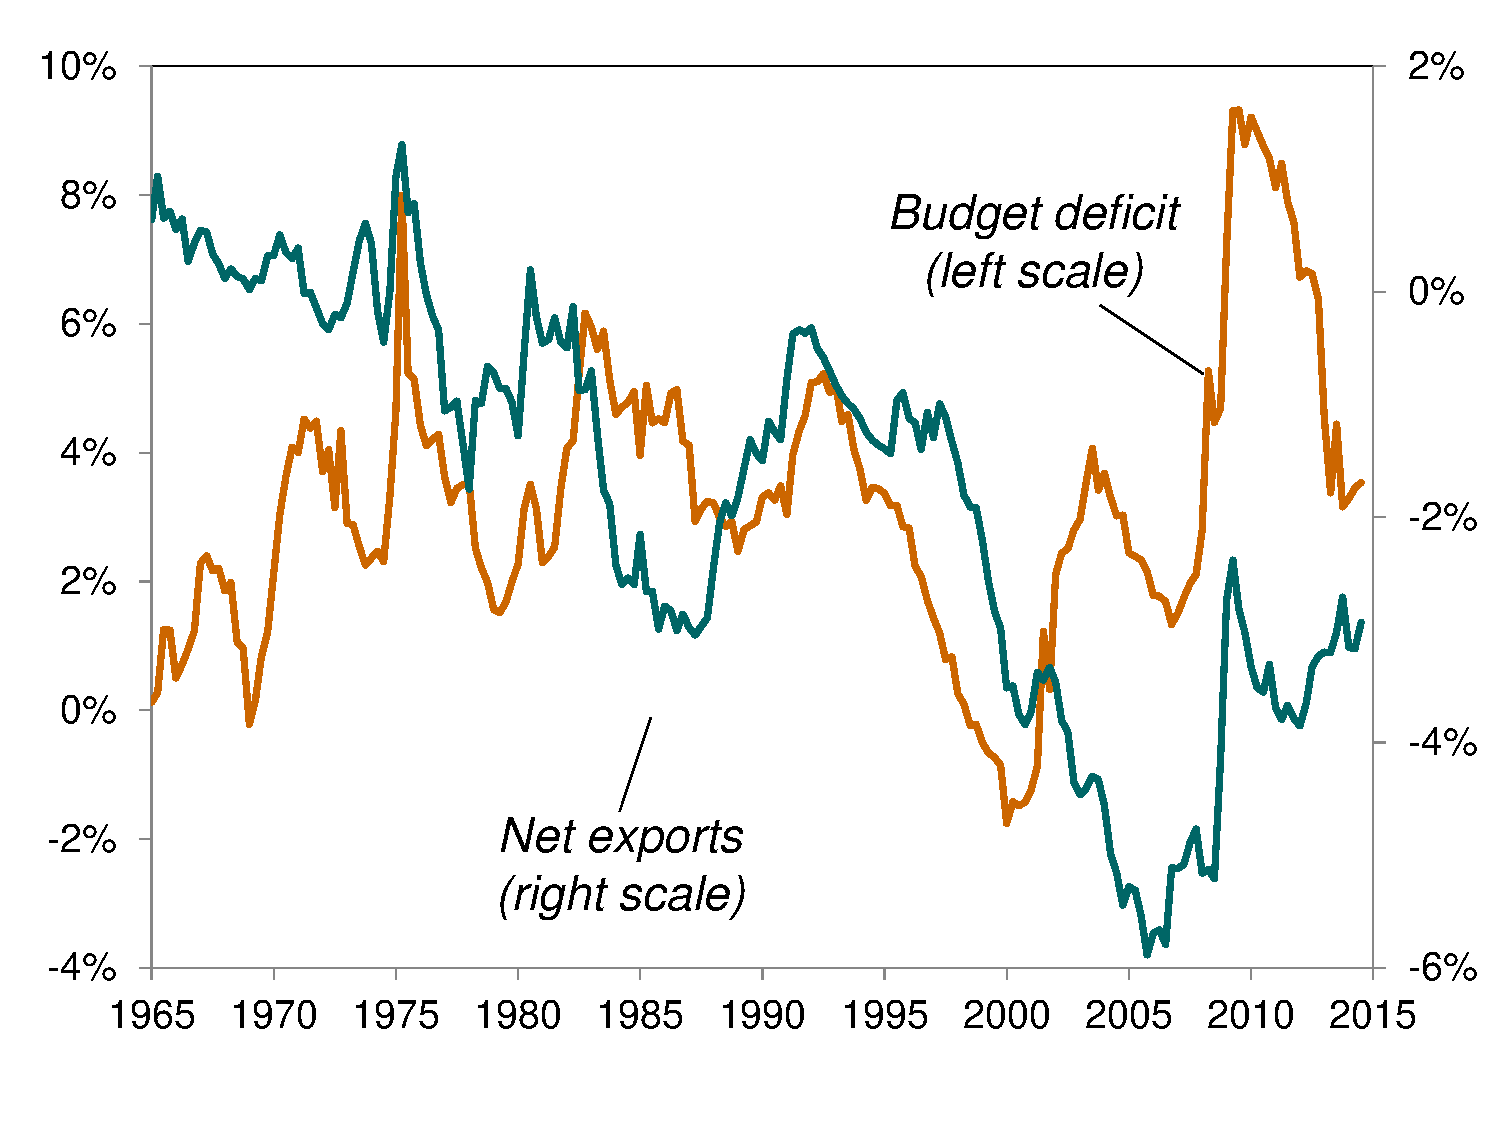
\includegraphics[height=3.1in,width=4.25in]{us_nx_budget.pdf}
\end{center}
\end{frame}


\end{document} 